\documentclass[a4j,xelatex,ja=standard,jafont=hiragino-pron, 9pt]{bxjsarticle}
% \documentclass[a4j, 9pt]{jsarticle}

\usepackage{graphicx}
\usepackage{frame}
\usepackage[dvips]{color}
\usepackage{float}
\let\origfigure=\figure
\let\endorigfigure=\endfigure
\renewenvironment{figure}[1][]{%
  \origfigure[H]
}{%
  \endorigfigure
}
\usepackage{listings}
\definecolor{Brown}{cmyk}{0,0.81,1,0.60}
\definecolor{OliveGreen}{cmyk}{0.64,0,0.95,0.40}
\definecolor{CadetBlue}{cmyk}{0.62,0.57,0.23,0}
\lstset{%
  language=R,
  stringstyle={\ttfamily},
  commentstyle={\itshape\color{Brown}},
  identifierstyle={\ttfamily\color{CadetBlue}\bfseries},
  keywordstyle={\ttfamily\color{OliveGreen}},
  basicstyle={\ttfamily},
  breaklines=true,
  columns=[l]{fullflexible},
  lineskip=-0.5pt,
  showstringspaces=ture,
  frame=single
}
\def\tightlist{\itemsep1pt\parskip0pt\parsep0pt}

\begin{document}
\section*{応用問題1}
\addcontentsline{toc}{section}{応用問題1}

\subsection*{(1)}\label{section}
\addcontentsline{toc}{subsection}{(1)}

最尤推定を用いて各都市ごとの回帰直線を求めると、次のような結果が得られた。

\begin{figure}
\centering
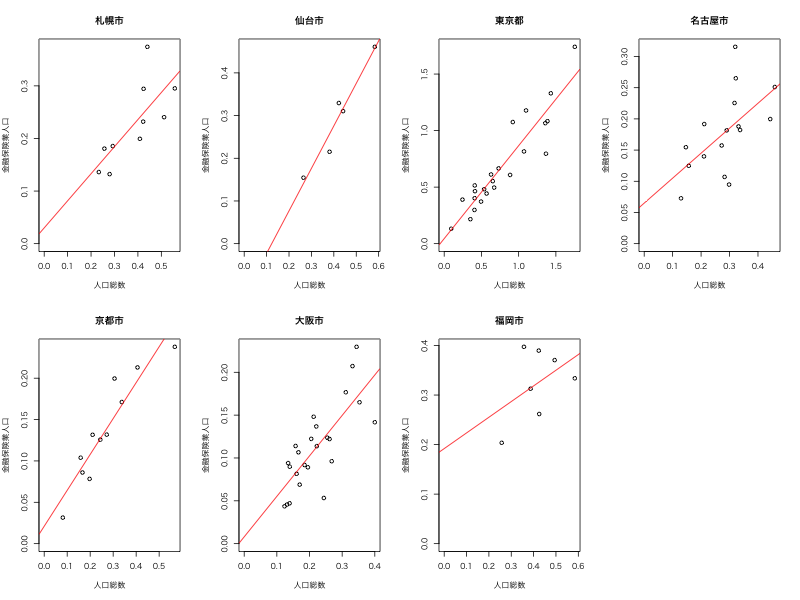
\includegraphics[width=14cm]{../src/output/image/regression.png}
\caption{最尤推定法による推定}
\end{figure}

これは次のスクリプトによって得られたものである。

\begin{lstlisting}
d <- read.csv("input/data_example1_fit.csv")
a.likelihood <- list()
b.likelihood <- list()

likelihood <- function(x) {
  prefecture <- subset(d, prefectures == x)
  H1 <- sum(prefecture$population^2)
  H2 <- sum(prefecture$population)
  H3 <- H2
  H4 <- length(prefecture$population)

  v1 <- sum(prefecture$population * prefecture$finance)
  v2 <- sum(prefecture$finance)

  H <- matrix(c(H1, H2, H3, H4), 2, 2)
  v <- matrix(c(v1, v2), 2, 1)

  HInv <- solve(H)

  HInv %*% v
}

for (x in 1:7) {
  a.likelihood[[x]] <- likelihood(x)[1]
  b.likelihood[[x]] <- likelihood(x)[2]
}
\end{lstlisting}

\subsection*{(2)}
\addcontentsline{toc}{subsection}{(2)}

階層ベイズ法を適用する際、まずStanというMCMCサンプラーを用いて推定した。

データから\(\sigma_Y\)、\(a\)、\(b\)、\(\sigma_a\)、\(\sigma_b\)を推定する。
\(Y\) は各年ごとのパラメータである。\(a\), \(b\) の平均を \(\hat{a}\),
\(\hat{b}\)とし、 \(\sigma_a\) と \(\sigma_b\) は \(a\) と \(b\)
を決めるハイパーパラメータとする。また、 \(PRE[n]\)
は各都市における値である。 Stanで書いたモデルのモデル式は次の通り。

\begin{eqnarray}
  Y[n] &\sim& Normal(b[PRE[n]] + a[PRE[n]] \times X[n], \sigma_Y) \\
  a[k] &\sim& Normal(\hat{a}, \sigma_a) \\
  b[k] &\sim& Normal(\hat{b}, \sigma_b)
\end{eqnarray}

この書き方は、「すべての都市の平均を \(\hat{a}\), であり、各都市の
\(a[k]\) は \(\hat{a}\)
を平均とした正規分布から生成された」という書き方になっている。\(\hat{b}\)
と \(b[k]\) についても同様である。

推定の結果、グラフと $a, b$ の値は次のようになった。

\begin{figure}
\centering
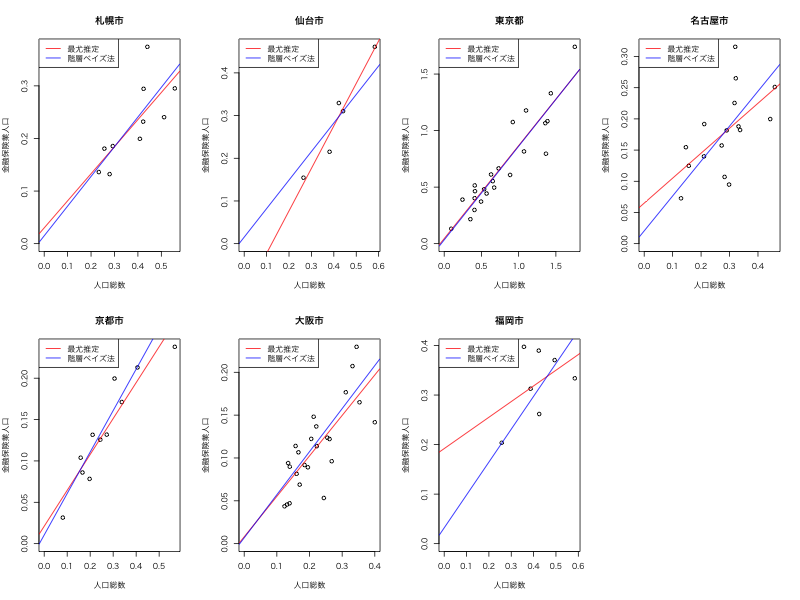
\includegraphics[width=15cm]{../src/output/image/mle-mcmc.png}
\caption{階層ベイズ法(ハミルトンモンテカルロ法)と最尤推定法の比較}
\end{figure}

\begin{figure}
  \centering
  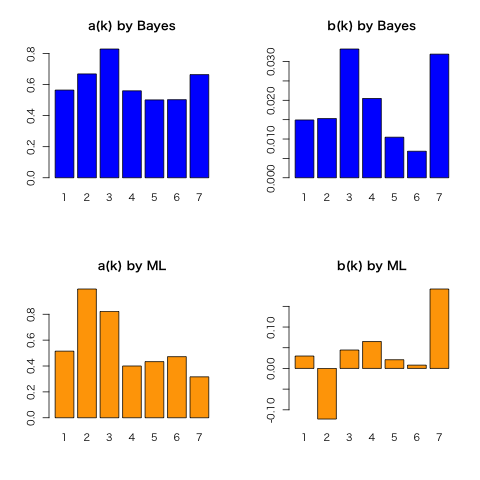
\includegraphics[width=8cm]{../../../Dropbox/B3-classes/DataAnalysis/report2/image/mle-bar.png}
  \caption{ハミルトンモンテカルロ法と最尤推定法の$a$ と $b$ の値の比較}
  \label{}
\end{figure}

また、講義で説明されたギブスサンプラー法を用いたサンプリングも試みた。その結果は次のようになった。

\begin{figure}
  \centering
  \includegraphics[width=15cm]{../../../Dropbox/B3-classes/DataAnalysis/report2/image/figure1.png}
  \caption{ギブスサンプラー法と最尤推定法の比較}
\end{figure}

\begin{figure}
  \centering
  \includegraphics[width=8cm]{../../../Dropbox/B3-classes/DataAnalysis/report2/image/figure2.png}
  \caption{ギブスサンプラー法と最尤推定法の $a$ と $b$ の比較}
  \label{}
\end{figure}

この2つの図を比較すると、ハミルトンモンテカルロ法の方がギブスサンプラー法より$b$の値が0に近づいていることから、
ハミルトンモンテカルロ法による階層ベイズ推定の方が収束の度合いが良いと考えられる。

\subsection*{(3)}
\addcontentsline{toc}{subsection}{(3)}

最も推定が大きく異なる都市は \textbf{福岡市}
である。考えられる原因は以下の通り、

\begin{enumerate}
\def\labelenumi{\arabic{enumi}.}
\tightlist
\item
  サンプル数が他の年に比べて少なく、ランダムネスによる影響が大きいため。
\item
  サンプルが少ない上に、点同士が反発しているような配置になっているため、よりランダムネスの影響を受けやすい(名古屋市も反発しているような配置になっているが、サンプル数が福岡市より多いため、最尤推定法と階層ベイズ法の差が福岡市に比べ小さいことより)。
\end{enumerate}

また、もっとも \(a(k)\) が大きい都市 \(k\) は \textbf{東京都} である。

\section*{応用問題2}
\addcontentsline{toc}{section}{応用問題2}

\subsection*{(1)}
\addcontentsline{toc}{subsection}{(1)}

次のRスクリプトで計算した結果、

\begin{itemize}
  \item
    平均$m_0 = 0.06476075$
  \item
    標準偏差$s_0 = 0.01153776$
\end{itemize}

となった。

\begin{lstlisting}
d <- read.csv('input/data_example2.csv')
X <- d$under15man / d$population
K <- 47
d <- transform(d, ratio=X)

variance <- function(x) var(x) * (length(x) - 1) / length(x)

m0 <- mean(X)
s0 <- sqrt(variance(X))
\end{lstlisting}

\subsection*{(2)}

\subsection*{(3)}



\end{document}
